\documentclass[12pt, titlepage]{article}

\usepackage{amsmath, mathtools}

\usepackage[round]{natbib}
\usepackage{amsfonts}
\usepackage{amssymb}
\usepackage{graphicx}
\usepackage{colortbl}
\usepackage{xr}
\usepackage{hyperref}
\usepackage{longtable}
\usepackage{xfrac}
\usepackage{tabularx}
\usepackage{float}
\usepackage{siunitx}
\usepackage{booktabs}
\usepackage{multirow}
\usepackage[section]{placeins}
\usepackage{caption}
\usepackage{fullpage}
\usepackage[letterpaper, portrait, margin=1in]{geometry}
\usepackage{helvet}
\usepackage{afterpage}
\usepackage{titlepic}
\usepackage[dvipsnames]{xcolor}

\usepackage{titlesec}
\titleformat{\section}{\large\bfseries\color{RedOrange}}{\rlap{\color{black}\rule[-0.3cm]{\linewidth}{1cm}} {\textcolor{RedOrange}{\thesection}}}{1em}{}

\renewcommand{\familydefault}{\sfdefault}

\hypersetup{
bookmarks=true,     % show bookmarks bar?
colorlinks=true,       % false: boxed links; true: colored links
linkcolor=red,          % color of internal links (change box color with linkbordercolor)
citecolor=blue,      % color of links to bibliography
filecolor=magenta,  % color of file links
urlcolor=cyan          % color of external links
}

\usepackage{array}

\externaldocument{../../SRS/SRS}

%% Comments

\usepackage{color}

\newif\ifcomments\commentstrue %displays comments
%\newif\ifcomments\commentsfalse %so that comments do not display

\ifcomments
\newcommand{\authornote}[3]{\textcolor{#1}{[#3 ---#2]}}
\newcommand{\todo}[1]{\textcolor{red}{[TODO: #1]}}
\else
\newcommand{\authornote}[3]{}
\newcommand{\todo}[1]{}
\fi

\newcommand{\wss}[1]{\authornote{blue}{SS}{#1}} 
\newcommand{\plt}[1]{\authornote{magenta}{TPLT}{#1}} %For explanation of the template
\newcommand{\an}[1]{\authornote{cyan}{Author}{#1}}

%% Common Parts

\newcommand{\progname}{ProgName} % PUT YOUR PROGRAM NAME HERE
\newcommand{\authname}{Team \#, Team Name
\\ Student 1 name and macid
\\ Student 2 name and macid
\\ Student 3 name and macid
\\ Student 4 name and macid} % AUTHOR NAMES                  

\usepackage{hyperref}
    \hypersetup{colorlinks=true, linkcolor=blue, citecolor=blue, filecolor=blue,
                urlcolor=blue, unicode=false}
    \urlstyle{same}
                                


\begin{document}

\title{\textbf{Module Interface Specification for \progname{}} \\ \vspace{2cm} 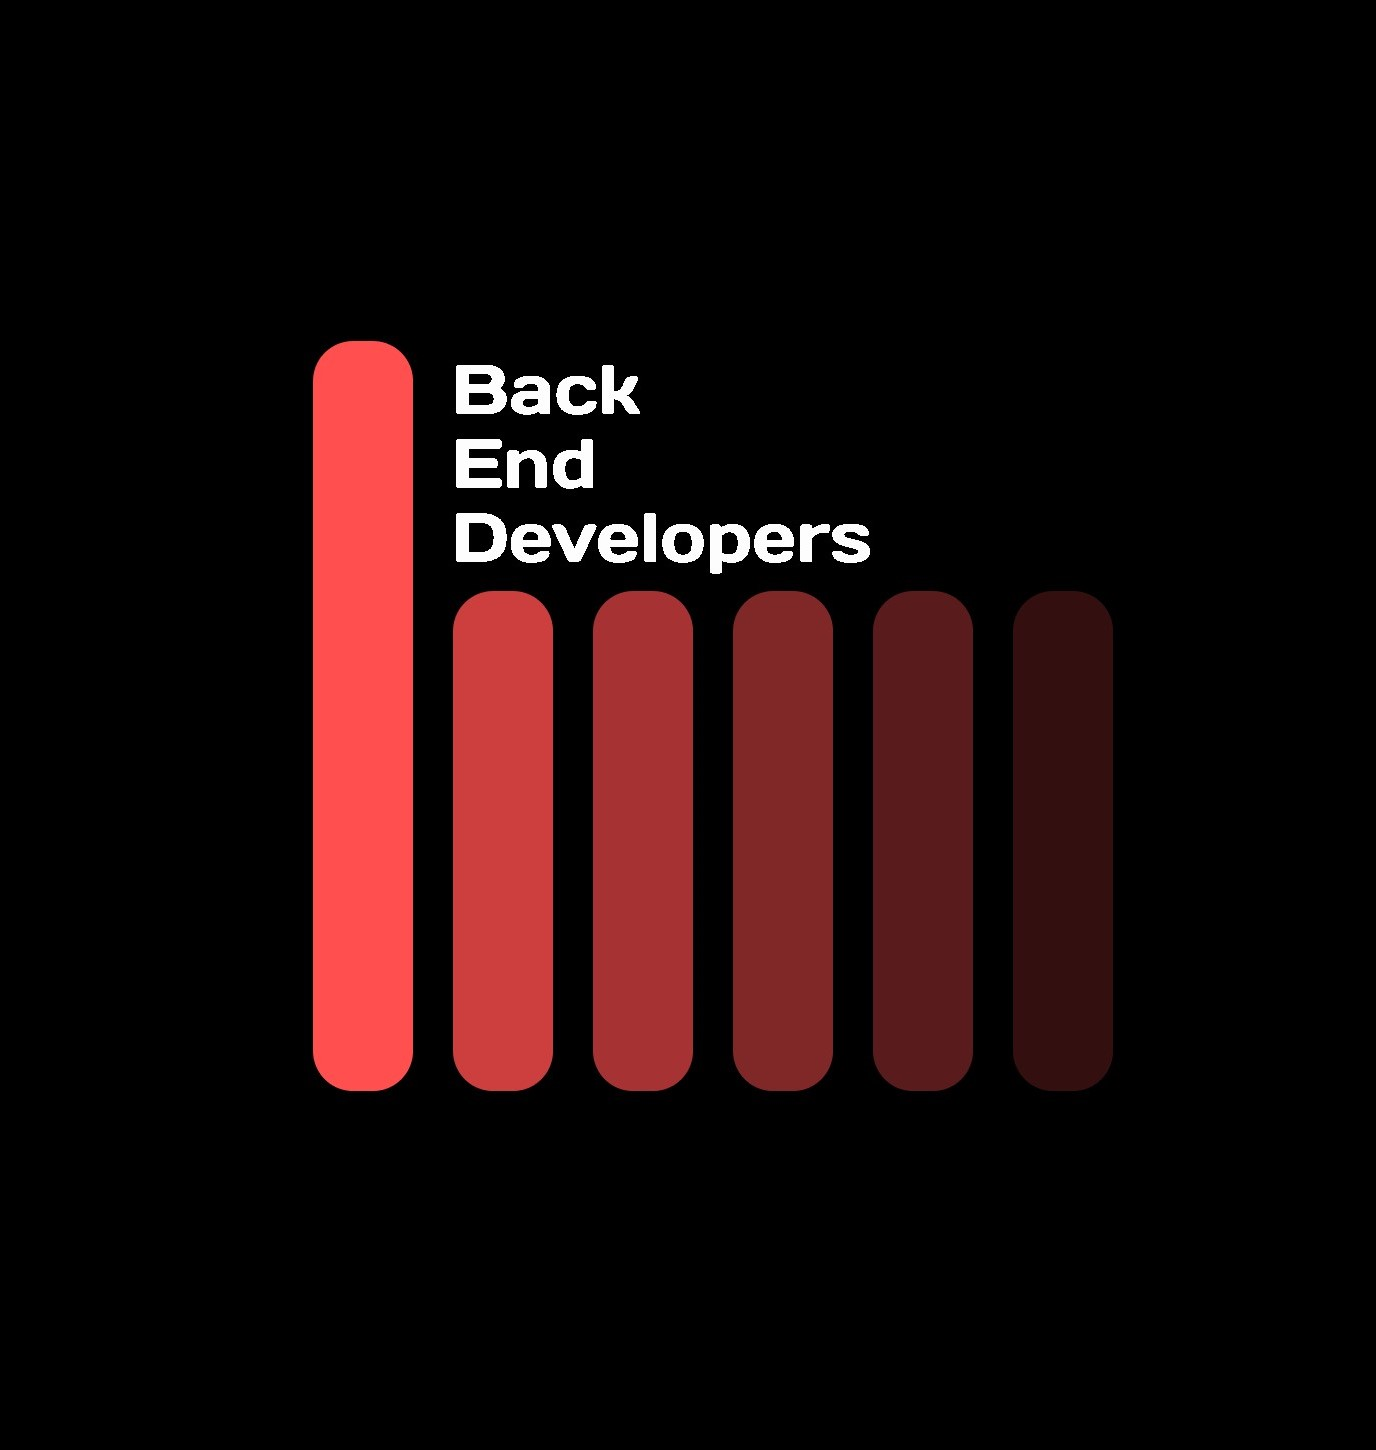
\includegraphics[width=0.5\textwidth]{../../logo.jpg}}
\author{\authname}

\date{\today}
 \pagecolor{black}\afterpage{\nopagecolor}
\color{white}\maketitle

\color{black}
\pagenumbering{roman}

\section{Revision History}

\begin{tabularx}{\textwidth}{p{3cm}p{2cm}X}
\toprule {\bf Date} & {\bf Version} & {\bf Notes}\\
\midrule
2023-01-18 & 1.0 & Initial documentation\\
2023-03-15 & 2.0 & Minor improvements and proof reading for revision 1\\
2023-04-03 & 2.1 & Incorporated TA feedback\\
2023-04-03 & 2.2 & Included logo and added style to the document\\
\bottomrule
\end{tabularx}

~\newpage

\section{Symbols, Abbreviations and Acronyms}

Please refer to the System Requirements Specifications document at \href{https://github.com/zakerl/Capstone_Project/blob/desDoc_Labeeb/docs/SRS/SRS.pdf}{this link} for relevant symbols, abbreviations.\\

\newpage

\tableofcontents

\newpage

\pagenumbering{arabic}

\section{Introduction}

The following document details the Module Interface Specifications for the EMAnator; the system currently being developed by the Back End Developers designed to aid in Ecological Momentary Assessment research. This document describes the various relevant details of interfacing with each module. These details include  module descriptions, the uses of each module, the syntax of each module, and the semantics associated with each module.\\

Complementary documents include the System Requirement Specifications and the Module Guide. The Back End Developers highly recommend a thorough read-through of each document prior to a reading of this document to attain the prerequisite knowledge necessary to fully understand this MIS. The System Requirements Specifications can be found at \href{https://github.com/zakerl/Capstone_Project/blob/main/docs/SRS/SRS.tex}{this link}, and the Module Guide can be found at \href{https://github.com/zakerl/Capstone_Project/blob/main/docs/Design/SoftArchitecture/MG.pdf}{this link}.

\section{Notation}

The structure of the MIS for modules comes from \citet{HoffmanAndStrooper1995},
with the addition that template modules have been adapted from
\cite{GhezziEtAl2003}.  The mathematical notation comes from Chapter 3 of
\citet{HoffmanAndStrooper1995}.  For instance, the symbol := is used for a
multiple assignment statement and conditional rules follow the form $(c_1
\Rightarrow r_1 | c_2 \Rightarrow r_2 | ... | c_n \Rightarrow r_n )$.

The following table summarizes the primitive data types used by \progname. 

\begin{center}
\renewcommand{\arraystretch}{1.2}
\noindent 
\begin{tabular}{l l p{7.5cm}} 
\toprule 
\textbf{Data Type} & \textbf{Notation} & \textbf{Description}\\ 
\midrule
Character & char & A single symbol or digit\\
Integer & $\mathbb{Z}$ & A number without a fractional component in (-$\infty$, $\infty$) \\
Natural number & $\mathbb{N}$ & A number without a fractional component in [1, $\infty$) \\
Real & $\mathbb{R}$ & Any number in (-$\infty$, $\infty$)\\
\bottomrule
\end{tabular} 
\end{center}

\noindent
The specification of \progname \ uses some derived data types: sequences, strings, and
tuples. Sequences are lists filled with elements of the same data type. Strings
are sequences of characters. Tuples contain a list of values, potentially of
different types. In addition, \progname \ uses functions, which
are defined by the data types of their inputs and outputs. Local functions are
described by giving their type signature followed by their specification.

\section{Module Decomposition}

The following table is taken directly from the Module Guide document for this project.
\begin{table}[h!]
  \centering
  \begin{tabular}{|p{0.3\textwidth} | p{0.3\textwidth} |p{0.3\textwidth}  |}
    \toprule
    \textbf{Level 1}        & \textbf{Level 2}        &\textbf{Level 3} \\
    \midrule

    \multirow{9}{0.3\textwidth} {Hardware-Hiding Module}              & Battery Management       & Battery\\
\cline{2-3}
					                                                          &  \multirow{2}{0.3\textwidth}{Data Storage}        & microSD     \\
																		&			&Database\\
\cline{2-3}
					                                                          & \multirow{3}{0.3\textwidth}{Sensor Array}         & Sensor Reading    \\
																		&			& Sensor Data Processing \\
																		&			& Sensor Prompt Validity \\ 
\cline{2-3}
												  & \multirow{2}{0.3\textwidth}{Physical Design} & Watch Straps \\
																		&			& Watch Case \\

    \midrule

    \multirow{3}{0.3\textwidth}{Behaviour-Hiding Module}  & Display System         & Display Screen  \\
\cline{2-3}
			                                                          & Prompt Generation       & Prompt Generation \\
\cline{2-3}
			                                                          & Real Time Clock      & RTC   \\


    \midrule

    \multirow{4}{0.3\textwidth}{Software Decision Module} &  \multirow{2}{0.3\textwidth}{Parameter Selection}& Create New User\\
																		&			& Configuration \\
\cline{2-3}
                                                          & \multirow{2}{0.3\textwidth}{Data Processing}       & Graph  \\
											&			& Data Display \\

    \bottomrule
  \end{tabular}
  \caption{Module Hierarchy}
  \label{TblMH}
\end{table}

\newpage

%%Main Window UI
%
%\section{MIS of Main Window UI Module} \label{Main Window UI Module} 
%
%\wss{You can reference SRS labels, such as R\ref{R_Inputs}.}
%
%\wss{It is also possible to use \LaTeX for hypperlinks to external documents.}
%
%\subsection{Module}
%
%Main Window \\
%
%\subsection{Uses}
%
%%Configuration (Section \ref{}), Create Records (Section \ref{}), View Records (Section \ref{}), Data View (Section \ref{})  \\
%Login (\ref{}) \\
%
%\subsection{Syntax}
%
%\subsubsection{Exported Constants}
%
%\subsubsection{Exported Access Programs}
%
%\begin{center}
%\begin{tabular}{p{2cm} p{4cm} p{4cm} p{2cm}}
%\hline
%\textbf{Name} & \textbf{In} & \textbf{Out} & \textbf{Exceptions} \\
%\hline
%\wss{accessProg} & - & - & - \\
%\hline
%\end{tabular}
%\end{center}
%
%\subsection{Semantics}
%
%\subsubsection{State Variables}
%
%\wss{Not all modules will have state variables.  State variables give the module
%  a memory.}
%
%\subsubsection{Environment Variables}
%
%\wss{This section is not necessary for all modules.  Its purpose is to capture
%  when the module has external interaction with the environment, such as for a
%  device driver, screen interface, keyboard, file, etc.}
%
%\subsubsection{Assumptions}
%
%\wss{Try to minimize assumptions and anticipate programmer errors via
%  exceptions, but for practical purposes assumptions are sometimes appropriate.}
%
%\subsubsection{Access Routine Semantics}
%
%\noindent \wss{accessProg}():
%\begin{itemize}
%\item transition: \wss{if appropriate} 
%\item output: \wss{if appropriate} 
%\item exception: \wss{if appropriate} 
%\end{itemize}
%
%\wss{A module without environment variables or state variables is unlikely to
%  have a state transition.  In this case a state transition can only occur if
%  the module is changing the state of another module.}
%
%\wss{Modules rarely have both a transition and an output.  In most cases you
%  will have one or the other.}
%
%\subsubsection{Local Functions}
%
%\wss{As appropriate} \wss{These functions are for the purpose of specification.
%  They are not necessarily something that is going to be implemented
%  explicitly.  Even if they are implemented, they are not exported; they only
%  have local scope.}
%
%
%%Login Window UI
%
%\newpage
%
%\section{MIS of Login Window UI} \label{Module} \wss{Use labels for
%  cross-referencing}
%
%\wss{You can reference SRS labels, such as R\ref{R_Inputs}.}
%
%\wss{It is also possible to use \LaTeX for hypperlinks to external documents.}
%
%\subsection{Module}
%
%\wss{Short name for the module}
%
%\subsection{Uses}
%
%
%\subsection{Syntax}
%
%\subsubsection{Exported Constants}
%
%\subsubsection{Exported Access Programs}
%
%\begin{center}
%\begin{tabular}{p{2cm} p{4cm} p{4cm} p{2cm}}
%\hline
%\textbf{Name} & \textbf{In} & \textbf{Out} & \textbf{Exceptions} \\
%\hline
%\wss{accessProg} & - & - & - \\
%\hline
%\end{tabular}
%\end{center}
%
%\subsection{Semantics}
%
%\subsubsection{State Variables}
%
%\wss{Not all modules will have state variables.  State variables give the module
%  a memory.}
%
%\subsubsection{Environment Variables}
%
%\wss{This section is not necessary for all modules.  Its purpose is to capture
%  when the module has external interaction with the environment, such as for a
%  device driver, screen interface, keyboard, file, etc.}
%
%\subsubsection{Assumptions}
%
%\wss{Try to minimize assumptions and anticipate programmer errors via
%  exceptions, but for practical purposes assumptions are sometimes appropriate.}
%
%\subsubsection{Access Routine Semantics}
%
%\noindent \wss{accessProg}():
%\begin{itemize}
%\item transition: \wss{if appropriate} 
%\item output: \wss{if appropriate} 
%\item exception: \wss{if appropriate} 
%\end{itemize}
%
%\wss{A module without environment variables or state variables is unlikely to
%  have a state transition.  In this case a state transition can only occur if
%  the module is changing the state of another module.}
%
%\wss{Modules rarely have both a transition and an output.  In most cases you
%  will have one or the other.}
%
%\subsubsection{Local Functions}
%
%\wss{As appropriate} \wss{These functions are for the purpose of specification.
%  They are not necessarily something that is going to be implemented
%  explicitly.  Even if they are implemented, they are not exported; they only
%  have local scope.}
%
%\newpage
%
%
%%Configuration UI
%
%\section{MIS of Login Window UI} \label{Module} \wss{Use labels for
%  cross-referencing}
%
%\wss{You can reference SRS labels, such as R\ref{R_Inputs}.}
%
%\wss{It is also possible to use \LaTeX for hypperlinks to external documents.}
%
%\subsection{Module}
%
%\wss{Short name for the module}
%
%\subsection{Uses}
%
%
%\subsection{Syntax}
%
%\subsubsection{Exported Constants}
%
%\subsubsection{Exported Access Programs}
%
%\begin{center}
%\begin{tabular}{p{2cm} p{4cm} p{4cm} p{2cm}}
%\hline
%\textbf{Name} & \textbf{In} & \textbf{Out} & \textbf{Exceptions} \\
%\hline
%\wss{accessProg} & - & - & - \\
%\hline
%\end{tabular}
%\end{center}
%
%\subsection{Semantics}
%
%\subsubsection{State Variables}
%
%\wss{Not all modules will have state variables.  State variables give the module
%  a memory.}
%
%\subsubsection{Environment Variables}
%
%\wss{This section is not necessary for all modules.  Its purpose is to capture
%  when the module has external interaction with the environment, such as for a
%  device driver, screen interface, keyboard, file, etc.}
%
%\subsubsection{Assumptions}
%
%\wss{Try to minimize assumptions and anticipate programmer errors via
%  exceptions, but for practical purposes assumptions are sometimes appropriate.}
%
%\subsubsection{Access Routine Semantics}
%
%\noindent \wss{accessProg}():
%\begin{itemize}
%\item transition: \wss{if appropriate} 
%\item output: \wss{if appropriate} 
%\item exception: \wss{if appropriate} 
%\end{itemize}
%
%\wss{A module without environment variables or state variables is unlikely to
%  have a state transition.  In this case a state transition can only occur if
%  the module is changing the state of another module.}
%
%\wss{Modules rarely have both a transition and an output.  In most cases you
%  will have one or the other.}
%
%\subsubsection{Local Functions}
%
%\wss{As appropriate} \wss{These functions are for the purpose of specification.
%  They are not necessarily something that is going to be implemented
%  explicitly.  Even if they are implemented, they are not exported; they only
%  have local scope.}
%
%\newpage
%
%
%%Create Records UI
%
%\section{MIS of Login Window UI} \label{Module} \wss{Use labels for
%  cross-referencing}
%
%\wss{You can reference SRS labels, such as R\ref{R_Inputs}.}
%
%\wss{It is also possible to use \LaTeX for hypperlinks to external documents.}
%
%\subsection{Module}
%
%\wss{Short name for the module}
%
%\subsection{Uses}
%
%
%\subsection{Syntax}
%
%\subsubsection{Exported Constants}
%
%\subsubsection{Exported Access Programs}
%
%\begin{center}
%\begin{tabular}{p{2cm} p{4cm} p{4cm} p{2cm}}
%\hline
%\textbf{Name} & \textbf{In} & \textbf{Out} & \textbf{Exceptions} \\
%\hline
%\wss{accessProg} & - & - & - \\
%\hline
%\end{tabular}
%\end{center}
%
%\subsection{Semantics}
%
%\subsubsection{State Variables}
%
%\wss{Not all modules will have state variables.  State variables give the module
%  a memory.}
%
%\subsubsection{Environment Variables}
%
%\wss{This section is not necessary for all modules.  Its purpose is to capture
%  when the module has external interaction with the environment, such as for a
%  device driver, screen interface, keyboard, file, etc.}
%
%\subsubsection{Assumptions}
%
%\wss{Try to minimize assumptions and anticipate programmer errors via
%  exceptions, but for practical purposes assumptions are sometimes appropriate.}
%
%\subsubsection{Access Routine Semantics}
%
%\noindent \wss{accessProg}():
%\begin{itemize}
%\item transition: \wss{if appropriate} 
%\item output: \wss{if appropriate} 
%\item exception: \wss{if appropriate} 
%\end{itemize}
%
%\wss{A module without environment variables or state variables is unlikely to
%  have a state transition.  In this case a state transition can only occur if
%  the module is changing the state of another module.}
%
%\wss{Modules rarely have both a transition and an output.  In most cases you
%  will have one or the other.}
%
%\subsubsection{Local Functions}
%
%\wss{As appropriate} \wss{These functions are for the purpose of specification.
%  They are not necessarily something that is going to be implemented
%  explicitly.  Even if they are implemented, they are not exported; they only
%  have local scope.}
%
%\newpage
%
%
%
%%View Records UI
%
%\section{MIS of Login Window UI} \label{Module} \wss{Use labels for
%  cross-referencing}
%
%\wss{You can reference SRS labels, such as R\ref{R_Inputs}.}
%
%\wss{It is also possible to use \LaTeX for hypperlinks to external documents.}
%
%\subsection{Module}
%
%\wss{Short name for the module}
%
%\subsection{Uses}
%
%
%\subsection{Syntax}
%
%\subsubsection{Exported Constants}
%
%\subsubsection{Exported Access Programs}
%
%\begin{center}
%\begin{tabular}{p{2cm} p{4cm} p{4cm} p{2cm}}
%\hline
%\textbf{Name} & \textbf{In} & \textbf{Out} & \textbf{Exceptions} \\
%\hline
%\wss{accessProg} & - & - & - \\
%\hline
%\end{tabular}
%\end{center}
%
%\subsection{Semantics}
%
%\subsubsection{State Variables}
%
%\wss{Not all modules will have state variables.  State variables give the module
%  a memory.}
%
%\subsubsection{Environment Variables}
%
%\wss{This section is not necessary for all modules.  Its purpose is to capture
%  when the module has external interaction with the environment, such as for a
%  device driver, screen interface, keyboard, file, etc.}
%
%\subsubsection{Assumptions}
%
%\wss{Try to minimize assumptions and anticipate programmer errors via
%  exceptions, but for practical purposes assumptions are sometimes appropriate.}
%
%\subsubsection{Access Routine Semantics}
%
%\noindent \wss{accessProg}():
%\begin{itemize}
%\item transition: \wss{if appropriate} 
%\item output: \wss{if appropriate} 
%\item exception: \wss{if appropriate} 
%\end{itemize}
%
%\wss{A module without environment variables or state variables is unlikely to
%  have a state transition.  In this case a state transition can only occur if
%  the module is changing the state of another module.}
%
%\wss{Modules rarely have both a transition and an output.  In most cases you
%  will have one or the other.}
%
%\subsubsection{Local Functions}
%
%\wss{As appropriate} \wss{These functions are for the purpose of specification.
%  They are not necessarily something that is going to be implemented
%  explicitly.  Even if they are implemented, they are not exported; they only
%  have local scope.}
%
%\newpage
%
%
%
%%Data View UI
%
%\section{MIS of Login Window UI} \label{Module} \wss{Use labels for
%  cross-referencing}
%
%\wss{You can reference SRS labels, such as R\ref{R_Inputs}.}
%
%\wss{It is also possible to use \LaTeX for hypperlinks to external documents.}
%
%\subsection{Module}
%
%\wss{Short name for the module}
%
%\subsection{Uses}
%
%
%\subsection{Syntax}
%
%\subsubsection{Exported Constants}
%
%\subsubsection{Exported Access Programs}
%
%\begin{center}
%\begin{tabular}{p{2cm} p{4cm} p{4cm} p{2cm}}
%\hline
%\textbf{Name} & \textbf{In} & \textbf{Out} & \textbf{Exceptions} \\
%\hline
%\wss{accessProg} & - & - & - \\
%\hline
%\end{tabular}
%\end{center}
%
%\subsection{Semantics}
%
%\subsubsection{State Variables}
%
%\wss{Not all modules will have state variables.  State variables give the module
%  a memory.}
%
%\subsubsection{Environment Variables}
%
%\wss{This section is not necessary for all modules.  Its purpose is to capture
%  when the module has external interaction with the environment, such as for a
%  device driver, screen interface, keyboard, file, etc.}
%
%\subsubsection{Assumptions}
%
%\wss{Try to minimize assumptions and anticipate programmer errors via
%  exceptions, but for practical purposes assumptions are sometimes appropriate.}
%
%\subsubsection{Access Routine Semantics}
%
%\noindent \wss{accessProg}():
%\begin{itemize}
%\item transition: \wss{if appropriate} 
%\item output: \wss{if appropriate} 
%\item exception: \wss{if appropriate} 
%\end{itemize}
%
%\wss{A module without environment variables or state variables is unlikely to
%  have a state transition.  In this case a state transition can only occur if
%  the module is changing the state of another module.}
%
%\wss{Modules rarely have both a transition and an output.  In most cases you
%  will have one or the other.}
%
%\subsubsection{Local Functions}
%
%\wss{As appropriate} \wss{These functions are for the purpose of specification.
%  They are not necessarily something that is going to be implemented
%  explicitly.  Even if they are implemented, they are not exported; they only
%  have local scope.}
%
%\newpage
%
%
%
%%Display Graphs UI
%
%\section{MIS of Login Window UI} \label{Module} \wss{Use labels for
%  cross-referencing}
%
%\wss{You can reference SRS labels, such as R\ref{R_Inputs}.}
%
%\wss{It is also possible to use \LaTeX for hypperlinks to external documents.}
%
%\subsection{Module}
%
%\wss{Short name for the module}
%
%\subsection{Uses}
%
%
%\subsection{Syntax}
%
%\subsubsection{Exported Constants}
%
%\subsubsection{Exported Access Programs}
%
%\begin{center}
%\begin{tabular}{p{2cm} p{4cm} p{4cm} p{2cm}}
%\hline
%\textbf{Name} & \textbf{In} & \textbf{Out} & \textbf{Exceptions} \\
%\hline
%\wss{accessProg} & - & - & - \\
%\hline
%\end{tabular}
%\end{center}
%
%\subsection{Semantics}
%
%\subsubsection{State Variables}
%
%\wss{Not all modules will have state variables.  State variables give the module
%  a memory.}
%
%\subsubsection{Environment Variables}
%
%\wss{This section is not necessary for all modules.  Its purpose is to capture
%  when the module has external interaction with the environment, such as for a
%  device driver, screen interface, keyboard, file, etc.}
%
%\subsubsection{Assumptions}
%
%\wss{Try to minimize assumptions and anticipate programmer errors via
%  exceptions, but for practical purposes assumptions are sometimes appropriate.}
%
%\subsubsection{Access Routine Semantics}
%
%\noindent \wss{accessProg}():
%\begin{itemize}
%\item transition: \wss{if appropriate} 
%\item output: \wss{if appropriate} 
%\item exception: \wss{if appropriate} 
%\end{itemize}
%
%\wss{A module without environment variables or state variables is unlikely to
%  have a state transition.  In this case a state transition can only occur if
%  the module is changing the state of another module.}
%
%\wss{Modules rarely have both a transition and an output.  In most cases you
%  will have one or the other.}
%
%\subsubsection{Local Functions}
%
%\wss{As appropriate} \wss{These functions are for the purpose of specification.
%  They are not necessarily something that is going to be implemented
%  explicitly.  Even if they are implemented, they are not exported; they only
%  have local scope.}
%
%\newpage

%%%%%%%%%%%%%%%%%%%%%%%

%%%%%%%%%%%%%%%%%%%%%%%

%%%% HARDWARE Interface Modules %%%%%



%Battery Management Module 

\section{MIS of Battery Module} \label{mBM} 

\subsection{Module}

Bat\_Man

\subsection{Uses}

None.

\subsection{Syntax}

\subsubsection{Exported Constants}
\begin{itemize}
\item BAT\_LOW\_THRESHOLD: $\mathbb{Z}$
\end{itemize}

\subsubsection{Exported Access Programs}

\begin{center}
\begin{tabular}{p{4cm} p{4cm} p{3cm} p{4cm}}
\hline
\textbf{Name} & \textbf{In} & \textbf{Out} & \textbf{Exceptions} \\
\hline
bed\_get\_bat\_level & - & battery\_level: $\mathbb{Z}$ & -\\
\hline
\end{tabular}
\end{center}

\subsection{Semantics}

\subsubsection{State Variables}

None.

\subsubsection{Environment Variables}

\begin{itemize}
\item battery\_level: $\mathbb{Z}$
\end{itemize}

\subsubsection{Assumptions}

System responds instantaneously to changes in flags (exported constants).

\subsubsection{Access Routine Semantics}

\begin{itemize}
\item bed\_get\_bat\_level: This function returns the battery voltage level as a percentage of the battery's full charge.
\end{itemize}

\subsubsection{Local Functions}
None.

\newpage

%Data Storage Module

\section{MIS of microSD Module} \label{mDS_1} 

\subsection{Module}

microSD\_Stor

\subsection{Uses}

Sensor Prompt Validity Module (Section \ref{mSA3}), Real Time Clock Module (Section \ref{mRTC})    %%%%%%%%%%%%

\subsection{Syntax}

\subsubsection{Exported Constants}

None.

\subsubsection{Exported Access Programs}

\begin{center}
\begin{tabular}{p{2cm} p{4cm} p{3.5cm} p{4cm}}
\hline
\textbf{Name} & \textbf{In} & \textbf{Out} & \textbf{Exceptions} \\
\hline
listDir & fs: type FS, dirname: char *, levels: $\mathbb{Z}$ & - & - \\
createDir & fs: type FS, path: char * & - & - \\
removeDir & fs: type FS, path: char * & - & - \\
\hline
\end{tabular}
\end{center}

\subsection{Semantics}

\subsubsection{State Variables}

None.

\subsubsection{Environment Variables}
\begin{itemize}
\item fs: type FS
\end{itemize}

\subsubsection{Assumptions}
\begin{itemize}
\item MicroSD card is formatted correctly.
\item MicroSD card is inserted correctly.
\end{itemize}
\subsubsection{Access Routine Semantics}

\begin{itemize}
\item listDir: This function lists all files in the path given.
\item createDir: This function creates a new folder at the designated path.
\item removeDir: This function removes a folder at the designated path.
\end{itemize}

\subsubsection{Local Functions}

\begin{center}
\begin{tabular}{p{2cm} p{4cm} p{3.5cm} p{4cm}}
\hline
\textbf{Name} & \textbf{In} & \textbf{Out} & \textbf{Exceptions} \\
\hline
readFile & fs: type FS, path: char * & - & - \\
writeFile & path: char * , message: char *& - & - \\
appendFile & fs: type FS, path: char * , message: char * & - & - \\
renameFile & fs: type FS, path1: char * , path2: char * & - & -\\
deleteFile & fs: type FS, path: char * & - & - \\
\hline
\end{tabular}
\end{center}

\subsubsection{FS Datatype Details}
The FS object as defined by the SD.h class.

\newpage

\section{MIS of Local Database Module} \label{mDS_2} 

\subsection{Module}

Database\_Stor

\subsection{Uses}

microSD Module (Section \ref{mDS_1})   %%%%%%%%%%%%

\subsection{Syntax}

\subsubsection{Exported Constants}

\begin{itemize}
\item MAX\_CHAR\_LIMIT: $\mathbb{Z}$
\item MAX\_FIRST\_NAME\_SIZE: $\mathbb{Z}$
\item MAX\_LAST\_NAME\_SIZE: $\mathbb{Z}$
\item MAX\_GENDER\_SIZE: $\mathbb{Z}$
\item MAX\_PHONE\_SIZE: $\mathbb{Z}$
\item MAX\_EMAIL\_SIZE: $\mathbb{Z}$
\item MAX\_ADDRESS\_SIZE: $\mathbb{Z}$
\item MAX\_DEVICE\_MODEL\_SIZE: $\mathbb{Z}$
\end{itemize}

\subsubsection{Exported Access Programs}

\begin{center}
\begin{tabular}{p{4cm} p{4cm} p{3.5cm} p{3.6cm}}
\hline
\textbf{Name} & \textbf{In} & \textbf{Out} & \textbf{Exceptions} \\
\hline
sqlite3.connect & database: type path-like & connection: type Connection & ProgrammingError: type Exception \\
conn.cursor & - & cursor: type Cursor & ProgrammingError: type Exception \\
cursor.execute & sql: char array & - & ProgrammingError: type Exception \\
conn.commit & - & - & ProgrammingError: type Exception \\
conn.close & - & - & ProgrammingError: type Exception \\
\hline
\end{tabular}
\end{center}

\subsection{Semantics}

\subsubsection{State Variables}

None.

\subsubsection{Environment Variables}

\begin{itemize}
\item FirstName: char array
\item LastName: char array
\item Gender: char array
\item PhoneNumber: char array
\item EmailID: char array
\item Address: char array
\item MonitoringPeriod: char array
\item TrackerModel: char array
\item Age: $\mathbb{Z}$
\item ParticipantID: $\mathbb{Z}$
\item StudyID: $\mathbb{Z}$
\item Weight: float
\item Height: float
\end{itemize}

\subsubsection{Assumptions}
None.
\subsubsection{Access Routine Semantics}
\begin{itemize}
\item sqlite3.connect: Performs a handshake between the database and the host software
\item conn.cursor: Establishes an object through which database transactions occur
\item cursor.execute: Executes the SQl statement to the database on the current transaction
\item conn.commit: Commits any pending transaction to the database
\item conn.close: Closes the database connection

\end{itemize}

\subsubsection{Local Functions}

None.

\subsubsection{path-like Datatype Details}
The path-like-object is an object which contains the string of the path to the .db database file

\subsubsection{Connection Datatype Details}
An object representing the sqlite3 object.

\subsubsection{Cursor Datatype Details}
An object which contains the functions which manipulate the database

\subsubsection{ProgrammingError Datatype Details}
A subclass of DatabaseError datatype.

\newpage

%Sensor Array Module

\section{MIS of Reading Sensor Module} \label{mSA1} 

\subsection{Module}

Sensor\_Reading

\subsection{Uses}

Battery Management (Section \ref{mBM})

\subsection{Syntax}

\subsubsection{Exported Constants}

\begin{itemize}
\item ACCEL\_SENSITIVITY: $\mathbb{Z}$
\item GYRO\_SENSITIVITY: $\mathbb{Z}$
\item Threshold: $\mathbb{Z}$
\item MPU\_CALIBRATION: $\mathbb{Z}$
\end{itemize}

\subsubsection{Exported Access Programs}
\begin{center}
\begin{tabular}{p{4cm} p{4cm} p{3.5cm} p{3.6cm}}
\hline
\textbf{Name} & \textbf{In} & \textbf{Out} & \textbf{Exceptions} \\
\hline
bed\_mpu\_detect & currentTime: $\mathbb{Z}$ & - & - \\
bed\_hr\_detect & - & - & - \\
\hline
\end{tabular}
\end{center}

\subsection{Semantics}

\subsubsection{State Variables}
\begin{itemize}
\item currentTime: $\mathbb{Z}$
\end{itemize}

\subsubsection{Environment Variables}
%interaction with device driver, screen, keyboard, file
\begin{itemize}
\item curr\_ax: $\mathbb{Z}$
\item curr\_ay: $\mathbb{Z}$
\item curr\_a$\mathbb{Z}$: $\mathbb{Z}$
\item curr\_gx: $\mathbb{Z}$
\item curr\_gy: $\mathbb{Z}$
\item curr\_g$\mathbb{Z}$: $\mathbb{Z}$
\end{itemize}

\subsubsection{Assumptions}
\begin{itemize}
\item All activity thresholds are provided from the configuration file.
\end{itemize}

\subsubsection{Access Routine Semantics}
\begin{itemize}
\item bed\_mpu\_detect: returns the current values of accelerometer and gyroscope.
\item bed\_hr\_detect: returns the current values of heart rate sensor.
\end{itemize}

\subsubsection{Local Functions}
\begin{center}
\begin{tabular}{p{4cm} p{4cm} p{3.5cm} p{3.6cm}}
\hline
\textbf{Name} & \textbf{In} & \textbf{Out} & \textbf{Exceptions} \\
\hline
bed\_mpu\_setup & - & b32\_err\_code: $\mathbb{Z}$ & b32\_err\_code: BED\_ERR\_MPU \\
bed\_hr\_setup & - & - & - \\
\hline
\end{tabular}
\end{center}

\newpage

\section{MIS of Sensor Data Processing Module} \label{mSA2} 

\subsection{Module}

Sensor\_Data

\subsection{Uses}

Sensor Reading (Section \ref{mSA1})

\subsection{Syntax}

\subsubsection{Exported Constants}
\begin{itemize}
\item ACTIVITY\_STEPS: $\mathbb{Z}$
\item ACTIVITY\_IDLE\_RESET: $\mathbb{Z}$
\item ACTIVITY\_IDLE\_WAIT: $\mathbb{Z}$
\end{itemize}

\subsubsection{Exported Access Programs}

\begin{center}
\begin{tabular}{p{4cm} p{1cm} p{4cm} p{4cm}}
\hline
\textbf{Name} & \textbf{In} & \textbf{Out} & \textbf{Exceptions} \\
\hline
bed\_mpu\_detect & currentTime: $\mathbb{Z}$ & - & - \\
bed\_hr\_detect & - & - & - \\
\hline
\end{tabular}
\end{center}

\subsection{Semantics}

\subsubsection{State Variables}
\begin{itemize}
\item currentTime: $\mathbb{Z}$
\end{itemize}

\subsubsection{Environment Variables}
%interaction with device driver, screen, keyboard, file
\begin{itemize}
\item step\_count: $\mathbb{Z}$
\item TOTAL\_STEP: $\mathbb{Z}$
\item step\_flag: $\mathbb{Z}$
\item activity\_flag: $\mathbb{Z}$
\end{itemize}
\subsubsection{Assumptions}

\begin{itemize}
\item There is space available in microSD card.
\end{itemize}

\subsubsection{Access Routine Semantics}
\begin{itemize}
\item bed\_mpu\_detect: returns the current values of accelerometer and gyroscope
\item bed\_hr\_detect: returns the current values of heart rate sensor
\end{itemize}
\subsubsection{Local Functions}

\begin{center}
\begin{tabular}{p{4cm} p{1cm} p{4cm} p{4cm}}
\hline
\textbf{Name} & \textbf{In} & \textbf{Out} & \textbf{Exceptions} \\
\hline
bed\_mpu\_setup & - & b32\_err\_code: $\mathbb{Z}$ & b32\_err\_code: BED\_ERR\_MPU\\
bed\_hr\_setup & - & - & -\\
\hline
\end{tabular}
\end{center}


\newpage


%Display System Module

\section{MIS of Display System Module} \label{mDS_2} 

\subsection{Module}

Disp\_Sys

\subsection{Uses}

Prompt Generation Module (Section \ref{mPG}), Real Time Clock Module (Section \ref{mRTC}), Battery Management (Section \ref{mBM})

\subsection{Syntax}

\subsubsection{Exported Constants}

\begin{itemize}
\item TEXT\_SI$\mathbb{Z}$E: $\mathbb{Z}$
\item BED\_TFT\_CS: $\mathbb{Z}$
\item BED\_TFT\_DC: $\mathbb{Z}$
\item BED\_TFT\_MOSI: $\mathbb{Z}$
\item BED\_TFT\_SCK: $\mathbb{Z}$
\end{itemize}

\subsubsection{Exported Access Programs}

\begin{center}
\begin{tabular}{p{3cm} p{3cm} p{3.5cm} p{4cm}}
\hline
\textbf{Name} & \textbf{In} & \textbf{Out} & \textbf{Exceptions} \\
\hline
bed\_display\_prompt & direction: $\mathbb{Z}$, prompt\_index: $\mathbb{Z}$, no\_of\_options: $\mathbb{Z}$, flag: $\mathbb{Z}$ & - & -  \\
bed\_display\_date\_time & - & - & - \\
\hline
\end{tabular}
\end{center}

\subsection{Semantics}

\subsubsection{State Variables}

\begin{itemize}
\item draw\_flag: $\mathbb{Z}$
\item wait\_flag: $\mathbb{Z}$
\end{itemize}

\subsubsection{Environment Variables}

\begin{itemize}
\item scroll\_index: $\mathbb{Z}$
\item curr\_hr: $\mathbb{Z}$
\item curr\_min: $\mathbb{Z}$
\item curr\_sec: $\mathbb{Z}$
\item prompt\_buff: char array
\item inPain: char array
\end{itemize}

\subsubsection{Assumptions}

None.

\subsubsection{Access Routine Semantics}

\begin{itemize}
\item bed\_display\_prompt: This function takes the type of prompt and prompt index and accordingly generates the corresponding questions and options. Upon answering all the questions, it will save the answers in the SD card.
\item bed\_display\_date\_time: This function grabs the current time and draws it to the screen.
\end{itemize}

\subsubsection{Local Functions}

\begin{center}
\begin{tabular}{p{3cm} p{3cm} p{3.5cm} p{4cm}}
\hline
\textbf{Name} & \textbf{In} & \textbf{Out} & \textbf{Exceptions} \\
\hline
bed\_init\_display & - & Response: string & BED\_ERR\_DISPLAY\_SYSTEM: $\mathbb{Z}$  \\
bed\_splash\_screen & - & - & - \\
bed\_display\_one\_line & displayText: char *, coordX: $\mathbb{Z}$, coordY: $\mathbb{Z}$, clearFlag: $\mathbb{Z}$ & - & -   \\
drawHour & - & - & - \\
drawMinute & - & - & -  \\
drawSecond & - & - & - \\
\hline
\end{tabular}
\end{center}


\newpage



%Prompt Generation Module

\section{MIS of Prompt Generation Module} \label{mPG} 

\subsection{Module}

Prompt\_Gen

\subsection{Uses}

Sensor Array Module (Section \ref{mSA2})

\subsection{Syntax}

\subsubsection{Exported Constants}
\begin{itemize}
\item MAX\_PROMPTS: $\mathbb{Z}$
\item WALK\_PROMPT\_SI$\mathbb{Z}$E: $\mathbb{Z}$
\item ALARM\_PROMPT\_SI$\mathbb{Z}$E: $\mathbb{Z}$
\item prompt\_test: type Prompt (struct)
\item prompt\_walking: type Prompt (struct)
\item prompt\_alarm: type Prompt (struct)
\end{itemize}

\subsubsection{Exported Access Programs}

None.

\subsection{Semantics}

\subsubsection{State Variables}

None.

\subsubsection{Environment Variables}

None.

\subsubsection{Assumptions}

None.

\subsubsection{Access Routine Semantics}

None.

\subsubsection{Local Functions}

None.

\subsubsection{Prompt Datatype Details}

\begin{itemize}
\item Prompt is a struct composed of 5 fields:
\item prompt\_id: $\mathbb{Z}$
\item no\_of\_options: $\mathbb{Z}$
\item prompt\_question: char array
\item prompt\_possible\_answers: char array (2D)
\item prompt\_response: char array
\end{itemize}

\newpage



%Real Time Clock Module

\section{MIS of Real Time Clock Module} \label{mRTC} 

\subsection{Module}

RTC

\subsection{Uses}

None.

\subsection{Syntax}

\subsubsection{Exported Constants}

\begin{itemize}
\item RTC\_ADDRESS: $\mathbb{Z}$
\item ALARM\_NUMBER: $\mathbb{Z}$
\item alarms: $\mathbb{Z}$ array (2D)
\item rtc: type RTC\_DS1307
\item now: type DateTime
\item daysOfTheWeek: char array (2D)
\item monthsOfTheYear: char array (2D)
\item rtc\_date\_time: type RTC\_DATE\_TIME
\end{itemize}

\subsubsection{Exported Access Programs}

\begin{center}
\begin{tabular}{p{3cm} p{3cm} p{2cm} p{4cm}}
\hline
\textbf{Name} & \textbf{In} & \textbf{Out} & \textbf{Exceptions} \\
\hline
bed\_display\_info & - & - & -  \\
bed\_alarm\_prompt & prev\_input: $\mathbb{Z}$ & new\_input: $\mathbb{Z}$ & - \\
bed\_set\_explicit\_date\_time & date: char *, time: char * & - & - \\
\hline
\end{tabular}
\end{center}

\subsection{Semantics}

\subsubsection{State Variables}
\begin{itemize}
\item alarm\_flag: $\mathbb{Z}$
\item curr\_alarm: $\mathbb{Z}$
\end{itemize}
\subsubsection{Environment Variables}

None.

\subsubsection{Assumptions}

\begin{itemize}
\item Initial date and time is correctly set.
\end{itemize}

\subsubsection{Access Routine Semantics}

\begin{itemize}
\item bed\_display\_info: This function grabs the current time from the DateTime struct, and stores it in the RTC\_DATE\_TIME struct.
\item bed\_alarm\_prompt: This function checks whether or not an alarm should be triggered based on the time, and accordingly updates the state.
\item bed\_set\_explicit\_date\_time: This function sets the date and time of the RTC explicitly.
\end{itemize}

\subsubsection{Local Functions}

\begin{center}
\begin{tabular}{p{3cm} p{3cm} p{2cm} p{4cm}}
\hline
\textbf{Name} & \textbf{In} & \textbf{Out} & \textbf{Exceptions} \\
\hline
bed\_init\_rtc & - & b32\_err\_code: $\mathbb{Z}$ & b32\_err\_code: BED\_ERR\_RTC\_SYSTEM \\
\hline
\end{tabular}
\end{center}

\subsubsection{RTC\_DATE\_TIME Datatype Details}

RTC\_DATE\_TIME is a struct composed of 6 fields:

\begin{itemize}
\item rtc\_year: $\mathbb{Z}$
\item rtc\_month: $\mathbb{Z}$
\item rtc\_day: $\mathbb{Z}$
\item rtc\_hour: $\mathbb{Z}$
\item rtc\_min: $\mathbb{Z}$
\item rtc\_sec: $\mathbb{Z}$
\end{itemize}

\subsubsection{RTC\_DS1307 Datatype Details}
The RTC object as defined by the RTClib system class.


\subsubsection{DateTime Datatype Details}
The DateTime object as defined by the RTClib system class.

\newpage


%Configuration Selection

\section{MIS of Configuration Module} \label{mPS2} 

\subsection{Module}

Config\_Param

\subsection{Uses}

MicroSD Module (Section \ref{mDS_1})

\subsection{Syntax}

\subsubsection{Exported Constants}

\begin{itemize}
\item MAX\_CHAR\_LIMIT: $\mathbb{Z}$
\item MAX\_FIRST\_NAME\_SI$\mathbb{Z}$E: $\mathbb{Z}$
\item MAX\_LAST\_NAME\_SI$\mathbb{Z}$E: $\mathbb{Z}$
\item MAX\_GENDER\_SI$\mathbb{Z}$E: $\mathbb{Z}$
\item MAX\_PHONE\_SI$\mathbb{Z}$E: $\mathbb{Z}$
\item MAX\_EMAIL\_SI$\mathbb{Z}$E: $\mathbb{Z}$
\item MAX\_ADDRESS\_SI$\mathbb{Z}$E: $\mathbb{Z}$
\item MAX\_DEVICE\_MODEL\_SI$\mathbb{Z}$E: $\mathbb{Z}$
\end{itemize}

\subsubsection{Exported Access Programs}

\begin{center}
\begin{tabular}{p{3cm} p{3cm} p{2cm} p{4cm}}
\hline
\textbf{Name} & \textbf{In} & \textbf{Out} & \textbf{Exceptions} \\
\hline
object.text & - & enter\_text: char array& - \\
\hline
\end{tabular}
\end{center}

\subsection{Semantics}

\subsubsection{State Variables}

\begin{itemize}
\item CreateRecord: type QPushButton
\end{itemize}

\subsubsection{Environment Variables}

\begin{itemize}
\item FirstName: char array
\item LastName: char array
\item Gender: char array
\item PhoneNumber: char array
\item EmailID: char array
\item Address: char array
\item MonitoringPeriod: char array
\item TrackerModel: char array
\item Age: $\mathbb{Z}$
\item ParticipantID: $\mathbb{Z}$
\item StudyID: $\mathbb{Z}$
\item Weight: float
\item Height: float
\end{itemize}


\subsubsection{Assumptions}

\begin{itemize}
\item All configuration parameters within acceptable limits.
\end{itemize}

\subsubsection{Access Routine Semantics}

\begin{itemize}
\item object.text: This function grabs what is typed into the UI input box and stores it into a variable
\end{itemize}

\subsubsection{Local Functions}

None.

\subsubsection{QPushButton Datatype Details}
The object from the PyQt class which enables UI buttons.

\newpage

\section{MIS of Graph Plotter} \label{mGP} 

\subsection{Module}

Graph\_Plot

\subsection{Uses}

Device Manager Module (Section \ref{mDM})

\subsection{Syntax}

\subsubsection{Exported Constants}

None.

\subsubsection{Exported Access Programs}

\begin{center}
\begin{tabular}{p{3cm} p{3cm} p{2cm} p{4cm}}
\hline
\textbf{Name} & \textbf{In} & \textbf{Out} & \textbf{Exceptions} \\
\hline
OpenHeart & - & - & - \\
OpenSteps & - & - & - \\
OpenActivity & - & - & - \\
sqlite3.connect & database: type path-like & connection: type Connection & ProgrammingError: type Exception \\
conn.cursor & - & cursor: type Cursor & ProgrammingError: type Exception \\
cursor.execute & sql: char array & - & ProgrammingError: type Exception \\
conn.commit & - & - & ProgrammingError: type Exception \\
conn.close & - & - & ProgrammingError: type Exception \\
\hline
\end{tabular}
\end{center}

\subsection{Semantics}

\subsubsection{State Variables}

\begin{itemize}
\item HeartGraph: type QPushButton
\item StepsGraph: type QPushButton
\item ActivityGraph: type QPushButton
\end{itemize}

\subsubsection{Environment Variables}

None.

\subsubsection{Assumptions}

\begin{itemize}
\item Data is in proper format and not corrupted.
\end{itemize}

\subsubsection{Access Routine Semantics}

\begin{itemize}
\item OpenHeart: This function fetches heart rate and time data from the database and plots it on the graph
\item OpenSteps: This function fetches step and time data from the database and plots it on the graph
\item OpenActivity: This function fetches activity and time data from the database and plots it on the graph
\item sqlite3.connect: Performs a handshake between the database and the host software
\item conn.cursor: Establishes an object through which database transactions occur
\item cursor.execute: Executes the SQl statement to the database on the current transaction
\item conn.commit: Commits any pending transaction to the database
\item conn.close: Closes the database connection
\end{itemize}

\subsubsection{Local Functions}

\begin{center}
\begin{tabular}{p{3cm} p{3cm} p{2cm} p{4cm}}
\hline
\textbf{Name} & \textbf{In} & \textbf{Out} & \textbf{Exceptions} \\
\hline
Plot & PlotTime: type Pandas Data Frame, Yaxis: type Pandas Data Frame, name: char array, color: char array & - & - \\
\hline
\end{tabular}
\end{center}


\subsubsection{QPushButton Datatype Details}
The object from the PyQt class which enables UI buttons.

\subsubsection{path-like Datatype Details}
The path-like-object is an object which contains the string of the path to the .db database file

\subsubsection{Connection Datatype Details}
An object representing the sqlite3 object

\subsubsection{Cursor Datatype Details}
An object which contains the functions which manipulate the database

\subsubsection{ProgrammingError Datatype Details}
A subclass of DatabaseError datatype.

\newpage

%Physical Design Module 

\section{MIS of Watch Case and Straps Module} \label{mPD} 

\subsection{Module}

Watch\_Case\_Strap

\subsection{Uses}

None.

\subsection{Syntax}


\subsubsection{Exported Constants}

None.

\subsubsection{Exported Access Programs}

None.

\subsection{Semantics}

Allow the device to be strapped onto the user.

\subsubsection{State Variables}

None.

\subsubsection{Environment Variables}

None.

\subsubsection{Assumptions}

Will not impact the functionality of any other components.

\subsubsection{Access Routine Semantics}

None.

\subsubsection{Local Functions}

None.

\newpage


\bibliographystyle {plainnat}
\bibliography {../../../refs/References}

\end{document}